\documentclass[hidelinks,12pt]{article}
\usepackage{algorithm2e}
\usepackage[brazil]{babel}
\usepackage[utf8]{inputenc}
\usepackage{listings}
\usepackage{amsmath}
\usepackage{amsfonts}
\usepackage{amssymb}
\usepackage{indentfirst}
\usepackage{caption}
\usepackage{color}
\usepackage{mathrsfs}
\usepackage{pgfplots}
\usepackage{hyperref}
\usepackage{fancyhdr}
\usepackage{verbatimbox}
\usepackage[export]{adjustbox}
\usepackage{xcolor}
\usepackage{textcomp}
\newcommand{\icon}[1]{\includegraphics[height=12pt]{#1}}
\newcommand{\bigicon}[1]{\includegraphics[height=50pt]{#1}}
% -------------------------------------------------------------------- %
% Cores para formatação de código
\usepackage{color}
\definecolor{vermelho}{rgb}{0.6,0,0} % para strings
\definecolor{verde}{rgb}{0.25,0.5,0.35} % para comentários
\definecolor{roxo}{rgb}{0.5,0,0.35} % para palavras-chaves
\definecolor{azul}{rgb}{0.25,0.35,0.75} % para strings
\definecolor{cinza-claro}{gray}{0.95}
% -------------------------------------------------------------------- %

% Declaracoes em Portugues
%\algrenewcommand\algorithmiccase{\textbf{caso}}


\DeclareCaptionFont{white}{\color{white}}
\DeclareCaptionFormat{listing}{%
	\parbox{\textwidth}{\colorbox{gray}{\parbox{\textwidth}{#1#2#3}}\vskip-4pt}}
\captionsetup[lstlisting]{format=listing,labelfont=white,textfont=white}
\lstset{frame=lrb,xleftmargin=\fboxsep,xrightmargin=-\fboxsep}


\newcommand{\iconb}[1]{\includegraphics[height=20pt]{#1}}
\setcounter{secnumdepth}{5}

\fancypagestyle{plain}{%
	\fancyfoot{}%
	\fancyhead{}%
}


\begin{document}
\pagenumbering{gobble}
\pagestyle{fancy}


\lhead{\bigicon{Figures/ufu}}
\chead{{\footnotesize UNIVERSIDADE FEDERAL DE UBERLÂNDIA \\ FACULDADE DE CIÊNCIA DA COMPUTAÇÃO \\ Construção de Compiladores} \\ \scriptsize{Av. João Naves de Ávila 2121, Campus Santa Mônica} }
\rhead{\bigicon{Figures/facom}}
\lfoot{}
\cfoot{}
\rfoot{}
\vspace*{8.5cm}
\begin{figure}[!h]
	\centering
	\Huge{\bf {Inteligência Computacional\\ Criptoaritmética}}
\end{figure}

\vspace*{6cm}

\noindent\textbf{Aluno:} Eduardo Costa de Paiva \qquad \textbf{Matrícula:} 11221BCC012 \\
\textbf{Email:} \texttt{\small \url{ eduardocspv@gmail.com}}\\
\textbf{Profº.:} Gina Maira Barbosa de Oliveira


\newpage
\fancyhead[C]{}
\fancyhead[R]{}
\fancyhead[L]{\leftmark}
\fancyfoot{}
%\fancyfoot[L]{{\footnotesize  Construção de Compiladores}}
\fancyfoot[C]{\hspace{1.5cm}\thepage}
%\fancyfoot[R]{{\footnotesize Universidade Federal de Uberlândia}}
\pagenumbering{arabic}


{\let\thefootnote\relax\footnotetext{\textit{UFU, Universidade Federal de Uberlândia, Minas Gerais, Brasil}}}

\newpage

\tableofcontents


\newpage

\section{Introdução}

	Esse relatório tem como objetivo a qualificação dos diferentes métodos de resolução de criptoaritmética utilizando algoritmo genéticos.  
	
	O sistema operacional que utilizado foi o Ubuntu 16.04 e a para o desenvolvimento foi utilizado a linguagem {\bf{C}}. Vale ressaltar que os tempos medidos estavam variando entre 1,4 1.6 segundos, mas após adicionar a funcionalidade para deixar as palavras genéricas este tempo aumentou.
	
	
\section{Testes realizados}

		
	\subsubsection{Testes com as possíveis combinações de técnicas para criptoaritmética: SEND+MORE=MONEY}
	
		
		\begin{figure}[h!]
		\centering
		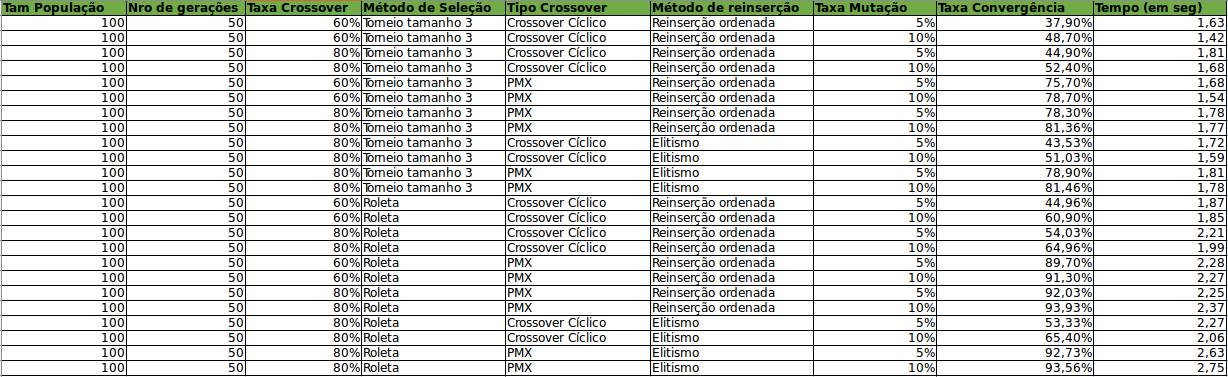
\includegraphics[scale=0.40]{Figures/1sendmoremoney}
		\caption{Testes com as possíveis combinações para SEND+MORE=MONEY}
		\end{figure}
	
	
	\subsubsection{Melhores resultados para SEND+MORE=MONEY}
	
		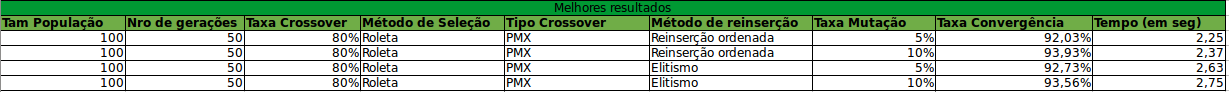
\includegraphics[width=\textwidth,height=\textheight,keepaspectratio]
		{Figures/melhoressendmoremoney.png}
		\begin{figure}[h!]
		\centering
		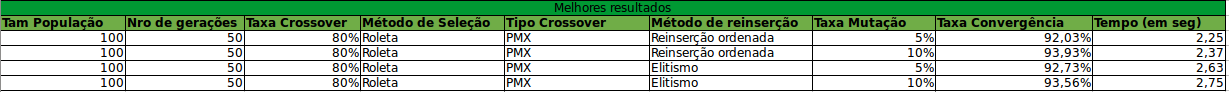
\includegraphics[scale=0.40]{Figures/melhoressendmoremoney}
		\caption{Melhores resultados para SEND+MORE=MONEY}
		\end{figure}
	
	\subsubsection{Testes utilizando melhores resultados para as demais criptoaritméticas}
	
		\begin{figure}[h!]
		\centering
		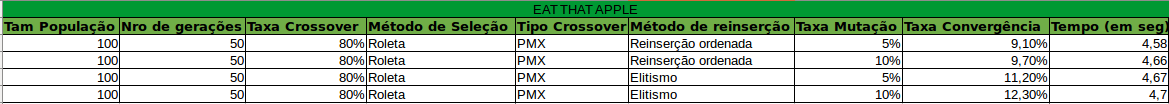
\includegraphics[scale=0.42]{Figures/eatthatapple}
		\caption{EAT + THAT = APPLE}
		\end{figure}
		
		\begin{figure}[h!]
		\centering
		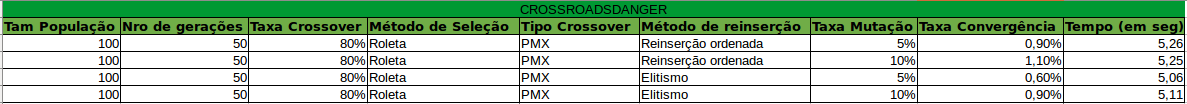
\includegraphics[scale=0.42]{Figures/crossroadsdanger}
		\caption{CROSS + ROADS = DANGER}
		\end{figure}
	
		\begin{figure}[h!]
		\centering
		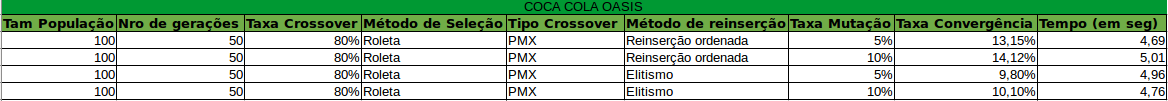
\includegraphics[scale=0.42]{Figures/cocacolaoasis}
		\caption{COCA + COLA = OASIS}
		\end{figure}
		\begin{figure}[h!]
		\centering
		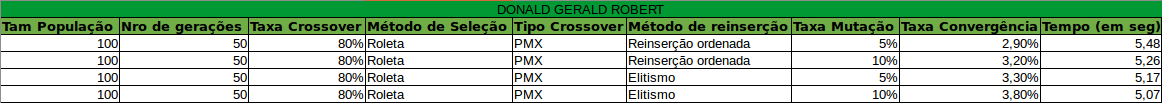
\includegraphics[scale=0.42]{Figures/donaldgeraldrobert}
		\caption{DONALD + GERALD = ROBERT}
		\end{figure}
		
		Para {\bf EAT+THAT = APPLE} a melhor configuração foi utilizando elitismo e mutação com taxa de 10\%
		
		
		Para {\bf CROSS+ROADS = DANGER } obteve-se pouca diferença entre os métodos. Mas a configuração utilizando elitismo e mutação de 10\% se sai bem ao olharmos tanto o tempo como convergência.
		
		
		Para {\bf COCA+COLA = OASIS} a melhor configuração foi utilizando reinserção ordenada e mutação com taxa de 10\%	
			
		
		Para {\bf DONALD+GERALD = ROBERT} a melhor configuração foi utilizando elitismo e mutação com taxa de 10\%
		
		
		\newpage
		{\bf Portanto, a melhor configuração observada foi:}
		\begin{enumerate}		
		\item Seleção: Roleta
		\item Crossover: PMX
		\item Reinserção: Elitismo
		\item Mutação: 10\%
		\end{enumerate}
		
		O crossover {\bf PMX} mistura bastante os genes de um indivíduo. A reinserção usando {\bf elitismo} preserva os melhores pais, além disso com a {\bf mutação} com a taxa de 10\% temos a garantia de termos uma diversidade maior da população. Portanto, a justificativa para ser uma boa configuração se dá pelo fato da maior diversidade e garantir a presença de pais com uma boa avaliação.
		
	\subsection{Aumento das taxas}
	
	
	Foi pedido, após verificar a melhor configuração, aumentar alguns valores para verificar se isso apresenta uma melhoria no algoritmo. Deve-se ter:
	\begin{itemize}
    \item População: 200 indivíduos
    
	\item Taxa de mutação: 15 \% maior que o valor atual
	
	\item Número de gerações: 100
	\end{itemize}
	\newpage
	\begin{figure}[h!]
		\centering
		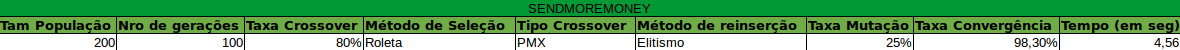
\includegraphics[scale=0.42]{Figures/aprimorandosendmoremoney}
		\caption{SEND+MORE = MONEY com nova configuração}
	\end{figure}
	
	\begin{figure}[h!]
		\centering
		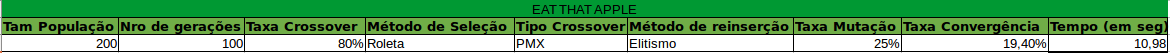
\includegraphics[scale=0.42]{Figures/aprimorandoeatthatapple}
		\caption{EAT+THAT=APPLE com nova configuração}
	\end{figure}
	
	\begin{figure}[h!]
		\centering
		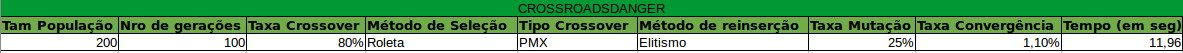
\includegraphics[scale=0.42]{Figures/aprimorandocrossroadsdanger}
		\caption{CROSS+ROADS=DANGER com nova configuração}
	\end{figure}
	
	
	\begin{figure}[h!]
		\centering
		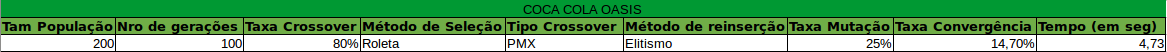
\includegraphics[scale=0.42]{Figures/aprimorandococacolaoasis}
		\caption{COCA+COLA=OASIS com nova configuração}
	\end{figure}
		
	\begin{figure}[h!]
		\centering
		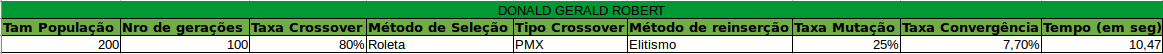
\includegraphics[scale=0.42]{Figures/aprimorandodonaldgeraldrobert}
		\caption{DONALD+GERALD=ROBERT com nova configuração}
	\end{figure}


	
	\justify
	Houve uma melhoria considerável, mas para a criptoaritmética CROSS + ROADS = DANGER a melhoria alcançada não compensou devido ao tempo de execução ter sido muito elevado.
	
	Uma mudança que poderia ser implementada para melhorar o desempenho seria uma condição para evitar crossover de pais que sejam iguais.
	
	
	\subsection{Alteração da função de avaliação}
	
	A nova função de avaliação proposta foi uma que considerasse a soma dígito a dígito.
\end{document}